%--------- Student instruction: change this by adding your neu id into the {}
\def\yourname{}
%-------------------------------------------------------------------------------------------------------------

%% ================= no need to edit any of this stuff
% --- no need to change anything in this section -----------------------------------------------------
\def\homework{1} % 0 for solution, 1 for problem-set only
\def\duedate{fri apr 22, 2022 at 11.59p}
\def\duelocation{via \href{https://gradescope.com/courses/331917}{gradescope}}
\def\hnumber{9}
\def\prof{abhi shelat}
\def\course{\href{https://shelat.khoury.neu.edu/22s-5800}{cs5800 algorithms s'22}}

\documentclass[11pt]{article}
%%% ==== standard installations of latex include all of the files that are referenced in this section.  However,
%%% ==== if you are having compile problems, consider commenting some of these commands out 
\usepackage[colorlinks,urlcolor=blue]{hyperref}
\usepackage[osf]{mathpazo}
\usepackage{amsmath,amsfonts,graphicx}
\usepackage{latexsym}
\usepackage[top=1in,bottom=1.3in,left=1.5in,right=1.5in,centering]{geometry}
\usepackage{color}
\usepackage{clrscode}
\definecolor{mdb}{rgb}{0.3,0.02,0.02} 
\definecolor{cit}{rgb}{0.05,0.2,0.45} 
\markboth{\yourname}{\yourname}
%%% ===================================================================


%%% ============ should be no need to edit anything in this section ====================
\newenvironment{proof}{\par\noindent{\it Proof.}\hspace*{1em}}{$\Box$\bigskip}
\newcommand{\qed}{$\Box$}
\newcommand{\alg}[1]{\mathsf{#1}}
\newcommand{\handout}{
   \renewcommand{\thepage}{H\hnumber-\arabic{page}}%
   \noindent%
   \begin{center}%
      \vbox{%
    \hbox to \columnwidth {\sc{\course} --- abhi shelat \hfill}%
    \vspace{-2mm}%
    \hbox to \columnwidth {\sc due \MakeLowercase{\duedate} \duelocation\hfill {\Huge\color{mdb}H\hnumber.\yourname}}%
      }
   \end{center}
   \vspace*{2mm}
}
\newcommand{\solution}[1]{\medskip\noindent\textbf{Solution:}#1}
\newcommand{\bit}[1]{\{0,1\}^{ #1 }}
\newtheorem{problem}{\sc\color{cit}problem}
\newtheorem{lemma}{Lemma}
\newtheorem{definition}{Definition}
%%% ===================================================================
\thispagestyle{empty}

\begin{document}\handout


\begin{problem}
Long stable matches
\end{problem}

We showed in class that the stable matching algorithm ends in $O(n^2)$ time with a stable match.  Find a set of preference inputs for 6 proposers and reviewers that requires at least 30 (in general, $n\cdot(n-1)$) proposals to be made before a stable matching is found no matter which order the proposals are made.  Your answer  should list the preferences of the proposers and the reviewers. 

\noindent\textbf{Solution:}\\

\noindent\textbf{Proposers:}
$$P_1 : R_1 \succ R_2 \succ R_3 \succ R_4 \succ R_5 \succ \textcolor{red}{R_6}$$
$$P_2 : R_2 \succ R_3 \succ R_4 \succ R_5 \succ \textcolor{red}{R_1} \succ R_6$$
$$P_3 : R_3 \succ R_4 \succ R_5 \succ R_1 \succ \textcolor{red}{R_2} \succ R_6$$
$$P_4 : R_4 \succ R_5 \succ R_1 \succ R_2 \succ \textcolor{red}{R_3} \succ R_6$$
$$P_5 : R_5 \succ R_1 \succ R_2 \succ R_3 \succ \textcolor{red}{R_4} \succ R_6$$
$$P_6 : R_1 \succ R_2 \succ R_3 \succ R_4 \succ \textcolor{red}{R_5} \succ R_6$$

\noindent\textbf{Reviewers:}
$$R_1 : \textcolor{red}{P_2} \succ P_3 \succ P_4 \succ P_5 \succ P_6 \succ P_1$$
$$R_2 : \textcolor{red}{P_3} \succ P_4 \succ P_5 \succ P_6 \succ P_1 \succ P_2$$
$$R_3 : \textcolor{red}{P_4} \succ P_5 \succ P_6 \succ P_1 \succ P_2 \succ P_3$$
$$R_4 : \textcolor{red}{P_5} \succ P_6 \succ P_1 \succ P_2 \succ P_3 \succ P_4$$
$$R_5 : \textcolor{red}{P_6} \succ P_1 \succ P_2 \succ P_3 \succ P_4 \succ P_5$$
$$R_6 : \textcolor{red}{P_1} \succ P_2 \succ P_3 \succ P_4 \succ P_5 \succ P_6$$

\noindent \textbf{Note:} The reviewers and proposers marked in \textcolor{red}{red} is one of the stable matching found using the algorithm.

\newpage




\begin{problem}Fair Tug of War
\end{problem}

Recall the Tug of War problem from DP homework.  Consider the closely related Fair Tug of War problem (FTW): given the non-negative weights of $n$ people, $W=(w_1,w_2,\ldots,w_n)$, divide the people into two teams, $L,R$, such that every person in $W$ is either in $L$ or in $R$, and such that $\sum_{\ell\in L} w_\ell = \sum_{r\in R} w_r$. In other words, the two teams include everyone, and both teams' weights sum to exactly the same value.  Note, the team sizes are not necessarily evenly split as was required in the Tug of War problem.

The subset sum problem is a famous NP-complete problem: given a list of non-negative numbers $L=(x_1,x_2,\ldots,x_n)$ and a target $t$, find a subset $S\subseteq L$ of numbers that sum to $t$, i.e., $\sum_{s\in S} s = t$.

Show that our Fair Tug of War problem is NP-complete.
\\

\noindent\textbf{Solution:}
For this, we show that $\proc{SubsetSum} \leq_{p} \proc{FairTugOfWar}$.

\begin{figure}[h]
\centering
    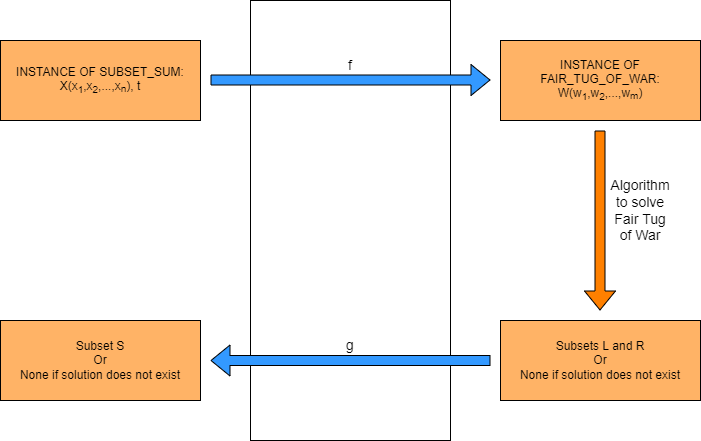
\includegraphics[width=100mm]{Q2.png}
\end{figure}

\noindent\textbf{Reduction from $\proc{SubsetSum}$ to $\proc{FairTugOfWar}$:}\\
Let $\bar{X} = \sum_{i = i}^{n} x_i$.
\begin{enumerate}
    \item if $\bar{X} = t$, then $\proc{SubsetSum}(X, t)$ reduces to  $\proc{FairTugOfWar(X)}$.
    \item else, let $x' = |\bar{X}-2t|$. Let $W = X \cup \{x'\}$, then $\proc{SubsetSum}(X, t)$ reduces to $\proc{FairTugOfWar}(W)$.
\end{enumerate}


\noindent\textbf{Proof:} Given $\proc{SubsetSum}(X, t)$, $3$ cases occur:
\begin{enumerate}
    \item $\mathbf{t = \frac{\bar{X}}{2}}$:\\
    Then the problem becomes the $\proc{FairTugOfWar}(X)$ directly as subsets $S\subseteq X$ and $X-S$ has $\sum_{s\in S} s = \sum_{s\in (X-S)} s= \frac{\bar{X}}{2}$.
    \item $\mathbf{t < \frac{\bar{X}}{2}}$ (Thus $\bar{X}-2t>0$):\\
    Thus, $x' = \bar{X}-2t$. Let $S\subseteq X$ be a solution of $\proc{SubsetSum}(X, t)$.\\ 
    Then $\sum_{s\in S} s = t$ and $\sum_{s\in (X-S)} s= \bar{X}-t$.\\
    Let $S' = S \cup {x'}$, then $\sum_{s\in S'} s = t + \bar{X}-2t = \bar{X} - t = \sum_{s\in (X-S)} s$.\\
    Thus the problem reduces to dividing $W = X \cup {x'}$ into two subsets with equal sum($=\bar{X} - t$), which is $\proc{FairTugOfWar(W)}$.
    \item $\mathbf{t > \frac{\bar{X}}{2}}$ (Thus $\bar{X}-2t<0$):\\
    Thus, $x' = 2t-{\bar{X}}$. Let $S\subseteq X$ be a solution of $\proc{SubsetSum}(X, t)$.\\ 
    Then $\sum_{s\in S} s = t$ and $\sum_{s\in (X-S)} s= \bar{X}-t$.\\
    Let $S' = (X-S) \cup {x'}$, then $\sum_{s\in S'} s = \bar{X}-t + 2t-\bar{X} = t = \sum_{s\in S} s$.\\
    Thus the problem again reduces to dividing $W = X \cup {x'}$ into two subsets with equal sum($=t$), which is $\proc{FairTugOfWar(W)}$.
\end{enumerate}

\noindent\textbf{Solution of $\proc{SubsetSum}(X,t) = S$ from solution of $\proc{FairTugOfWar}(W) = (L,R)$:}
\begin{enumerate}
    \item If solution of $\proc{FairTugOfWar}(W)$ does not exist, then solution of $\proc{SubsetSum}(X,t)$ also does not exist.
    \item If $t = \frac{\bar{X}}{2}$, then $S$ can either be $L$ or $R$.
    \item If $t < \frac{\bar{X}}{2}$, let $L$ be the subset containing element $x'$. Then $S = L - {x'}$.
    \item If $t > \frac{\bar{X}}{2}$, let $L$ be the subset containing element $x'$. Then $S = R$.
\end{enumerate}

\noindent\textbf{Proof:}
\begin{enumerate}
    \item We were able to convert an instance of $\proc{SubsetSum}(X, t)$ to $\proc{FairTugOfWar}(W)$. Thus, if $\proc{SubsetSum}(X, t)$ has a solution, if and only if $\proc{FairTugOfWar}(W)$ also has a solution.
    \item If $t = \frac{\bar{X}}{2}$, then $\sum_{s \in L} s= \sum_{s \in R} s= \frac{\bar{X}}{2} = t$. Thus $S=L$ or $S=R$.
    \item If $t < \frac{\bar{X}}{2}$, $\sum_{s \in L} s= X - t$.\\
    Then, $\sum_{s \in L-{x'}} s = X - t - (X - 2t) = t$. Thus $S = L - {x'}$. 
    \item If $t > \frac{\bar{X}}{2}$, $\sum_{s \in R} s= t$ and since $R$ does not contain $x'$, so $S = R$.
\end{enumerate}


Both Reduction and Solution Conversion can be done in $\Theta(n)$ time.

\newpage

\begin{problem} Ministry of Museums (20pts Extra Credit) \end{problem}

\noindent The ministry of museums wants to ensure that every town either has a museum or is next to a town that has a museum.  Given a map of a country consisting of towns and roads between them, the {\em Museum} problem is to decide whether
$k$ museums can be placed in towns so as to satisfy the Ministry's goal.

\medskip

\noindent Let language $L = \left\{ (G,k) \ \left|  \ \parbox{3in}{ $G$ is a graph, and $k$ museums can be placed at verticies such that every vertex either has a museum or is adjacent to one  with a museum.} \right.\right\}$.

\begin{enumerate}
    \item Argue that $L \in NP$. (Recall, this means showing that it is easy to verify an instance in polynomial time given a witness.)

    \item Next show that $L$ is NP-complete by showing a reduction from one of the NP-complete problems we discussed in class.
    
\end{enumerate}
\noindent\textbf{Solution:}
\begin{enumerate}
    \item Let $S$ be the set of towns having museums. We can verify whether $S$ is a solution of $\proc{Museum}(G(V, E),k)$ using the following algorithm:
    \begin{codebox}
        \Procname{$\proc{VerifyMuseum}(G(V, E),k,S)$}
        \li \textbf{if} $|S| \neq k$
        \li \quad \textbf{return} $False$
        \li \textbf{for all} $v \in V$
        \li \quad \textbf{if} $v \notin S$ \textbf{and} $\forall u \in adj(v)$, $u \notin S$
        \li \quad \quad \textbf{return} $False$
        \li \textbf{return} True
        \end{codebox}
    
    $\proc{VerifyMuseum}(G(V, E),k,S)$ checks if for all towns $v \in V$, either $v$ has a museum or any of its neighbours have museum and returning $True$ only if all of the towns satisfy this condition.
    
    The time complexity for $\proc{VerifyMuseum}$ is $\Theta(E)$ since each pair $(u,v) \in V$ connected by roads are checked atmost twice. Since we can verify whether $S$ is a solution of $\proc{Museum}(G(V, E),k)$ in a polynomial time, $\proc{Museum} \in NP$.
    \newpage
    \item For this, we show that $\proc{Clique} \leq_{p} \proc{Museum}$.
        
    \begin{figure}[h]
    \centering
        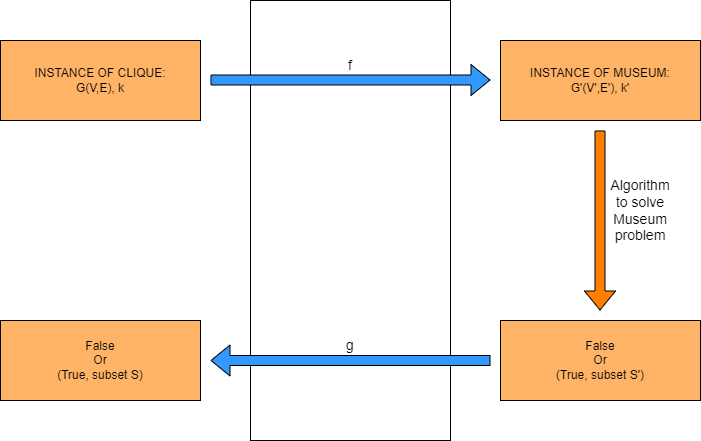
\includegraphics[width=100mm]{Q3.png}
    \end{figure}
    
    \noindent\textbf{Reduction from $\proc{Clique}(G(V, E),k)$ to $\proc{Museum}(G'(V', E'),k')$:}\\
    Let $G^c(V, E^c)$ be a graph such that for every vertices $u,v \in V$, if $e(u,v) \notin E$ then $e(u,v) \in E^c$.\\
    $G$ has a $k$-Clique iff $G^c$ has a solution to $k$-Museum.\\
    $\proc{Clique}(G(V, E),k)$ can be reduced to $\proc{Museum}(G^c(V, E^c),k)$
    
    \noindent\textbf{Proof:}\\
    Let $S \subseteq V$ be a solution to $\proc{Clique}(G(V, E),k)$. $|S| = k$.\\
    Consider any vertex $v \in V-S$. Then there exists a vertex $u \in S$ such that $e(u, v) \notin E$.\\
    Thus $e(u,v) \in E^c$.\\
    It means that $v$ is connected to atleast one vertex $u \in S$ in $G^c$. Since $|S| = k$, we have a subset of $V$ in $G^c$ such that $\forall v \in V$, either $v \in S$ or $\exists u \in adj(v)$ such that $u \in S$. Hence $S$ is a solution of $\proc{Museum}(G^c(V, E^c),k)$.
    
    
    
    
    
    
    
    
    
    
    % \noindent\textbf{Solution of $\proc{Museum}(X,t) = S$ from solution of $\proc{Clique}(W) = (L,R)$:}
    
    
    % \noindent\textbf{Proof:}
\end{enumerate}



\end{document}